%----------------------------------------------------------------------------------------
%	PACKAGES AND DOCUMENT CONFIGURATIONS
%----------------------------------------------------------------------------------------
\documentclass[11pt]{article}
\usepackage{amsmath} % Required for some math elements
\usepackage{hyperref}
\usepackage[table,xcdraw]{xcolor}
\usepackage{lipsum} 
\usepackage{cite}
\usepackage{graphicx} % Required for the inclusion of images
\usepackage{algorithmic}
\usepackage{array}
\usepackage{adjustbox}
\usepackage{bookmark}
\usepackage{mcode}
\usepackage[margin=24mm]{geometry}


\interdisplaylinepenalty=2500 %Note that the amsmath package sets \interdisplaylinepenalty to 10000 thus preventing page breaks from occurring within multiline equations. Use: \interdisplaylinepenalty=2500 after loading amsmath to restore such page breaks as IEEEtran.cls normally does

\hypersetup{ %color attributes of citation, link, etc.
    colorlinks=orange,
    linkcolor=cyan,
    filecolor=gray,      
    urlcolor=cyan,
    citecolor=cyan,
}
%----------------------------------------------------------------------------------------
%	DOCUMENT INFORMATION
%----------------------------------------------------------------------------------------
\title{RESE412 - Project 2 Report \\ Renewable Energy Control Systems}
\author{Daniel Eisen}
\date{\today}

\begin{document}
\maketitle
%----------------------------------------------------------------------------------------
%	DOCUMENT CONTENT
%----------------------------------------------------------------------------------------
\section{Introduction}
This project and report describes the process of exploring and implementing a Demand Side Management Control System on a previously modelled and sized solar based microgrid. The only focus of the designed system was the shift/alter the behaviour and power draw of the hot water cylinders within each of the houses.

\section{Background and Motivation}
    \subsection*{Demand Side Management}
    Demand-side Management of an energy is a method based on modifying the end-user/energy consumers energy demand needs, using various methods, such that this behavioural change result in meeting a set of requirements. 

    These methods can be split into direct control; direct modification of energy consuming elements of the grid, and indirect control; such of financial incentive etc that work to encourage end user behaviour change.

    \subsection*{Motivation and Approach}
    This project takes the direct control approach by implementing an in situ control system to modify the energy consumption dynamics each houses hot water cylinders. This was the focus due to the inherent load/consumption misalignment of peak solar production and the morning/evening demand of hot water. 
    
    To more concretely define the goal(s) of this system:
    \begin{itemize}
        \item Water must still meet T\_HIGH\_WH, set required hot water temperature once a day.
        \item Maintain (or improve) the total percentage of serviced load (taken across sample week)
        \item Allow for a reduction in storage size required to meet load and therefore reduce microgrid cost 
    \end{itemize}

    Due to this the system will focus of Load Shifting the demand to better line up with available unused peak production, and avoid clipping to still meet the same total demand of the microgrid.

\newpage
\section{Uncontrolled Microgrid}
    The uncontrolled system is a 4 home, centrally supplied, solar generation based microgrid. 
    \begin{table}[h!]
        \begin{adjustbox}{width=\textwidth}
            \begin{tabular}{lllllll}
                \multicolumn{7}{c}{\cellcolor[HTML]{FFC7CE}{\color[HTML]{9C0006} Uncontrolled}}                                                                                                            \\
                \textbf{Turbine (kW)} & \textbf{turbine cost (\$)} & \textbf{storage (Ah)} & \textbf{storage cost (\$)} & \textbf{Total cost (\$)} & \textbf{unserviced (\%)} & \textbf{WH Bat Draw (\%)} \\
                52                    & \$135,200.00               & 460                    & \$103,040.00               & \$238,240.00             & 1.545                    & 63.04                    
            \end{tabular}
        \end{adjustbox}
        \caption{Sizing and Costing of Uncontrolled Microgrid}
        \label{tab:unc}
    \end{table}

    Table \ref{tab:unc} show the full relevant specification if the installation, with the main points of interest being the percentage of the water heaters drawn power being $63.04\%$ from the batteries, that minimum storage requirement of 460Ah (doubled in costing to preserve longevity) and the total cost of $\$238,240.00$. The load curve and battery levels across and model winter week as seen in \ref{fig:uncontrolled_load} and show delivery failure at battery drainage points.

    
    \begin{figure}[h!]
        \centering
        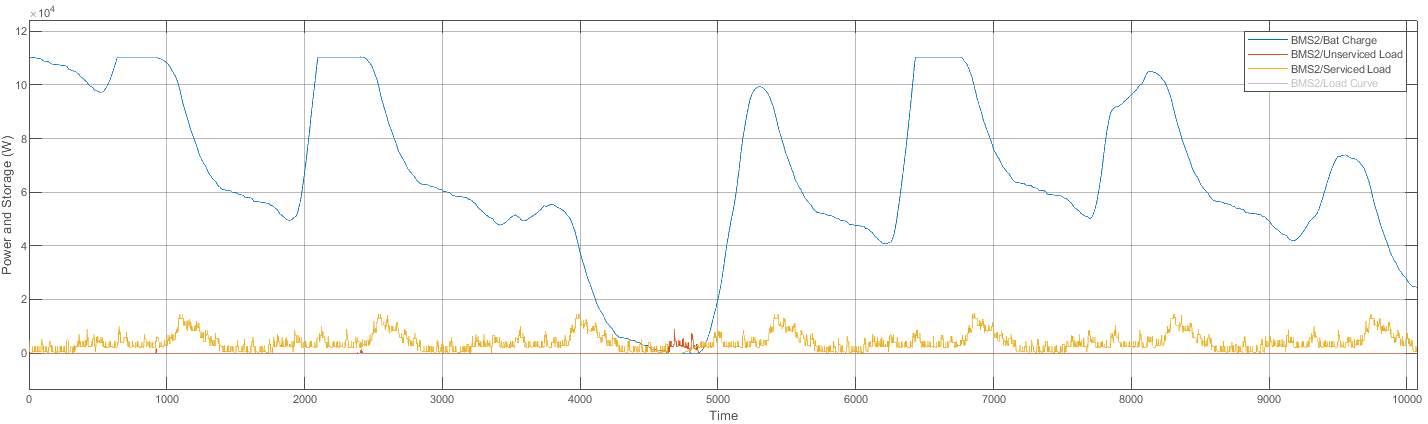
\includegraphics[width=\textwidth]{inc/uncontrolled_charge.png}
        \caption{}
        \label{fig:uncontrolled_load}
    \end{figure}
    
    In this uncontrolled state, the water heaters follow a thermostatic model. With the power draw being controlled with an internal thermostat that have a minimum and maximum temperature and bound between the two over the day with changing temperatures due to water use a cooling.\\
    Figure \ref{fig:unc_temps} shows the temperature characteristics under this system, note the relatively flat behaviour and reactive measures not anticipatory measure that the system can only take.

    \begin{figure}[h!]
        \centering
        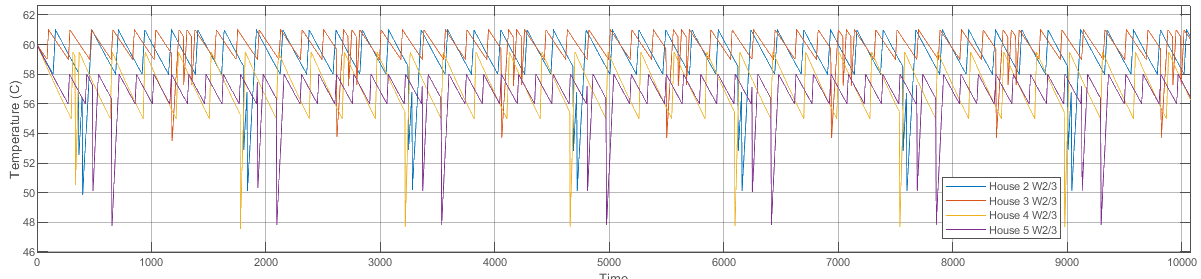
\includegraphics[width=\textwidth]{inc/uncontrolled_temps.png}
        \caption{Temperatures of uncontrolled water heats}
        \label{fig:unc_temps}
    \end{figure}

    
    
\section{Controlled Microgrid}
    \subsection{Topology}
    The chosen topology for the design of this Control System was a majority distributed system, in that each house has its own internal controller that modifies that power delivered to that houses cylinder. It incorporated an element of a more hybrid approach by a relying on a shared input between all the controllers that represents the remaining energy available (and capable) of supplying power to \textbf{all} the heaters. This external input great;y increases the robustness of the system, ensuring 1 house does not brown out the others. 
    
    This approach was done do the speed that it could be developed, as each of the internal controllers is identical and just relies on getting unique input from its house and the accuracy of the externally calculated available power.
    \subsection{Algorithm}
    The first part of the algorithm is the external input; Available Unused Power. This is calculated using a provided helper block that provides sum solar usage of the water heaters.
    $$unused = (available\;Solar-Panel\;Output)+Water\;Heater\;Draw$$

    The Water heater draw from the panel is added back the unused power is because that power should be made known as available to the controller and thus prevent the case of the controller "ringing" the power to the heaters because it thinks the power it just allocated depleted the unused power.
    
    As the aim of this system to maximally utilise solar power and minimise battery load, the thermostat of each house was modified to reach a max of 100 degrees Celsius when heating. This was done as it allow for less heating cycles per day, possibly allowing for a particularly good generation day to provide for 2 consecutive days with minimal intervention.

    The controller then makes use of a buck converter to vary the power delivered to the heaters by varying the delivered voltage. It does this by producing a duty cycle (0.0 to 1.0) as a function of the input used power and the max power draw of the cylinder itself. See \ref{ap:matlab} and the equation below descripting the limiting of power when unused power was less than max draw:
    
    $$D = unused/HW_{power}$$

    At this stage the controller only delivers power to the heaters when there is available otherwise unused solar, and ramps up the power delivery to match the panel output at that time. Where it fails is that it has no idea of if has met its temperature requirement that day, or if the sun if insufficient it lacks a bypass to the battery storage.

    With the use of persistent variables in MATLAB the controller can keep track of if the cylinder has met T\_HIGH each day and if it has not, then it defaults a 100\% duty cycle until it has reached T\_HIGH. It does not stop at 100 to better conserve battery stores and only meets what is required and specified per household. 100 degrees is only available in excess production. 

\newpage
\section{Results and Comparison}
    With the full implementation of the above described design, the system was simulated over the same model week as set by the uncontrolled system and the same data collected for comparison.

\begin{figure}[h!]
    \centering
    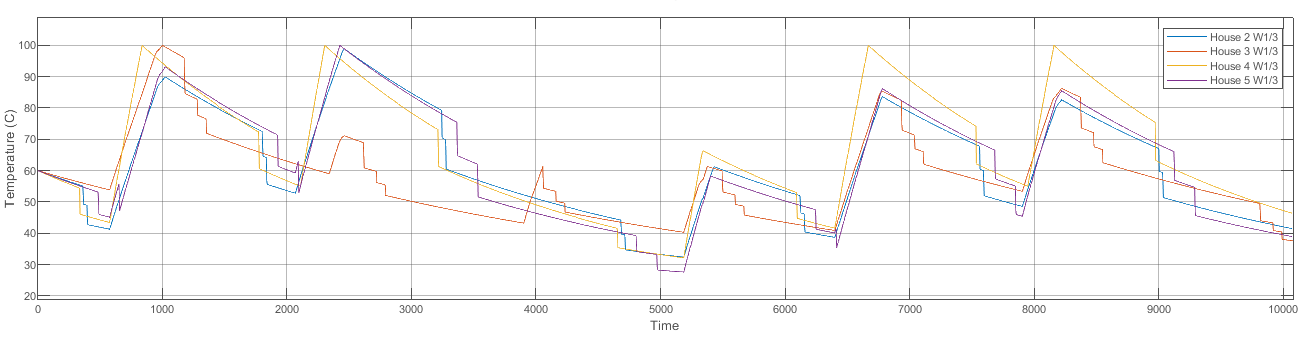
\includegraphics[width=\textwidth]{inc/controlled_temps.png}
    \caption{cylinder temperature}
    \label{fig:con_temps}
\end{figure}

The first evaluation criteria that would mediately render the system debunk were if it failed to meet temperature requirements. Figure \ref{fig:con_temps} shows that the bypass trigger in conjunction with over heating (100 degrees) \textbf{always} ensures that if there is available power from either the panels or batteries, that the water meets it requirement at least once per 24hrs. This does not however mean that it required heating everyday, as seen on the 3rd and final days.

\begin{figure}[h!]
    \centering
    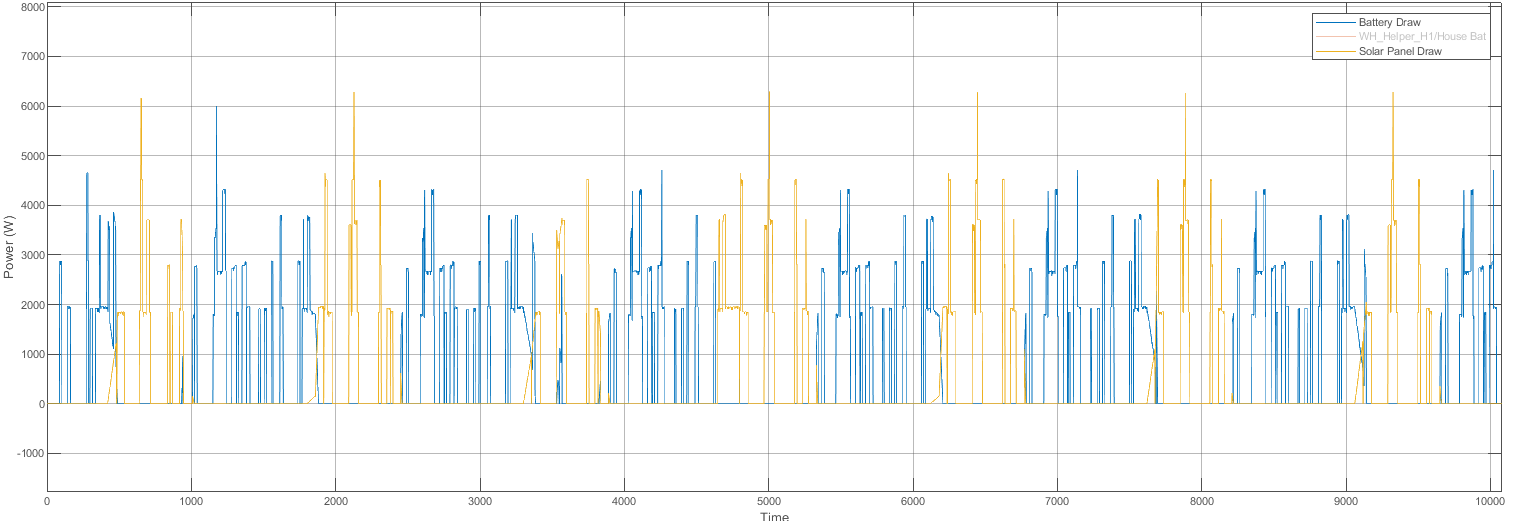
\includegraphics[width=\textwidth]{inc/uncontrolled_WH_draw.png}
    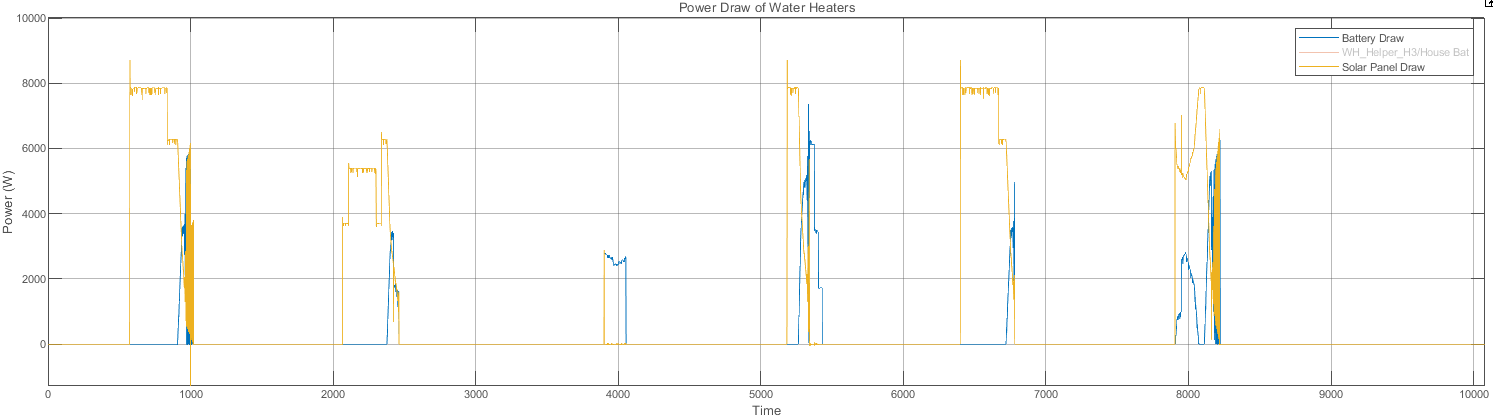
\includegraphics[width=\textwidth]{inc/controlled_WH_draw.png}
    \caption{Top: Uncontrolled water heater draw      Bottom: Controlled Draw}
    \label{fig:bat_wh}
\end{figure}

\newpage
One of the motivations of the system of the better utilise excess solar and reduced the draw from the storage in off-peak hours. Figure \ref{fig:bat_wh} shows that power draw shift as well as the load accumulation as compared to the uncontrolled system. This greater illustrated/quantified as 49.07\% decrease in battery draw to meet water heater demand. Figure \ref{fig:power_distributed} shows the full effect of the redistribution and better utilisation of unused solar during peak production.


\begin{figure}[h!]
    \centering
    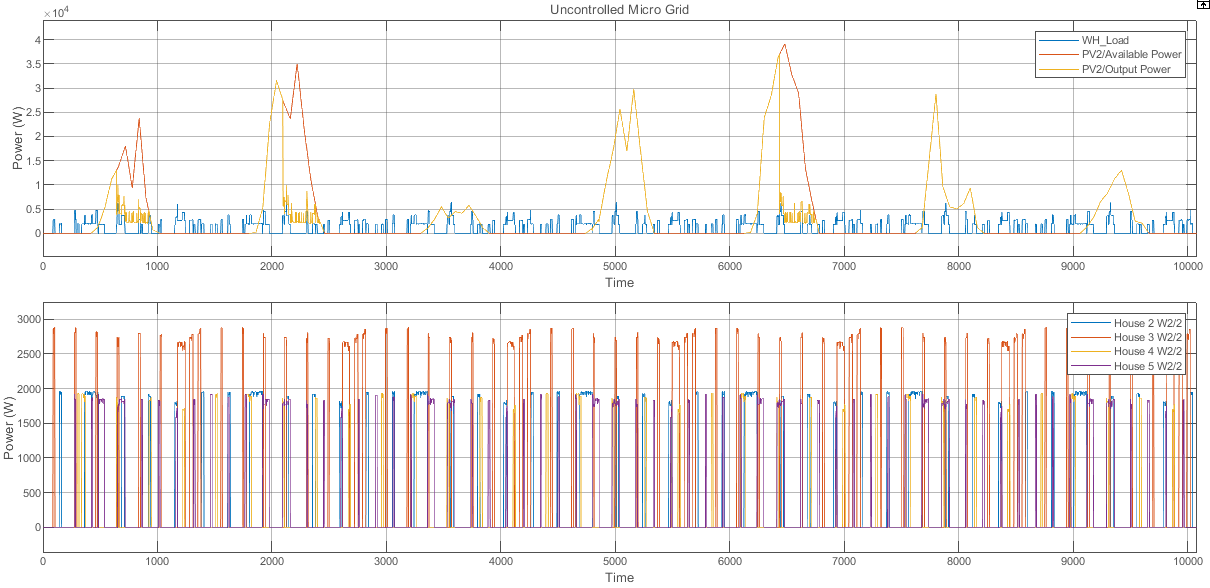
\includegraphics[width=\textwidth]{inc/uncontrolled_load_.png}   
    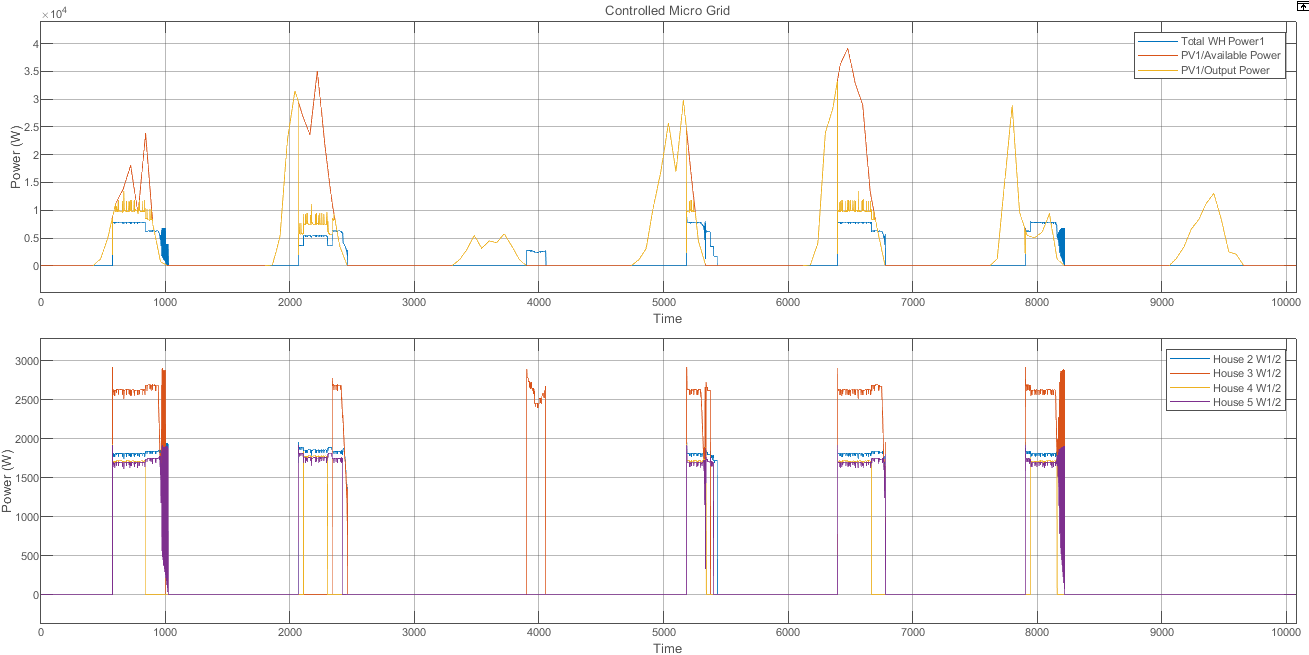
\includegraphics[width=\textwidth]{inc/controlled_load_.png}    
    \caption{}
    \label{fig:power_distributed}
\end{figure}



\newpage
\section{Conclusion}

\begin{table}[h!]
    \begin{adjustbox}{width=\textwidth}
        \begin{tabular}{lllllll}
            \multicolumn{7}{c}{\cellcolor[HTML]{C6EFCE}{\color[HTML]{006100} Controlled}}                                                                                                              \\
            \textbf{Turbine (kW)} & \textbf{turbine cost (\$)} & \textbf{storage (Ahr)} & \textbf{storage cost (\$)} & \textbf{Total cost (\$)} & \textbf{unserviced (\%)} & \textbf{WH Bat Draw (\%)} \\
            52                    & \$135,200.00               & 360                    & \$80,640.00                & \$215,840.00             & 5.67E-07                 & 18.97                    
        \end{tabular}
    \end{adjustbox}
\end{table}

The new final sized microgrid, incorporating the DSM control system, not only achieved its goal of better redestroying heater load, reducing battery reliance and hence required sized from 460Ah to 360Ah (possibly less) that facilitates as 20,000 dollar saving while upholding heating integrity and still reducing overall unserved load.

\begin{figure}[h!]
    \centering
    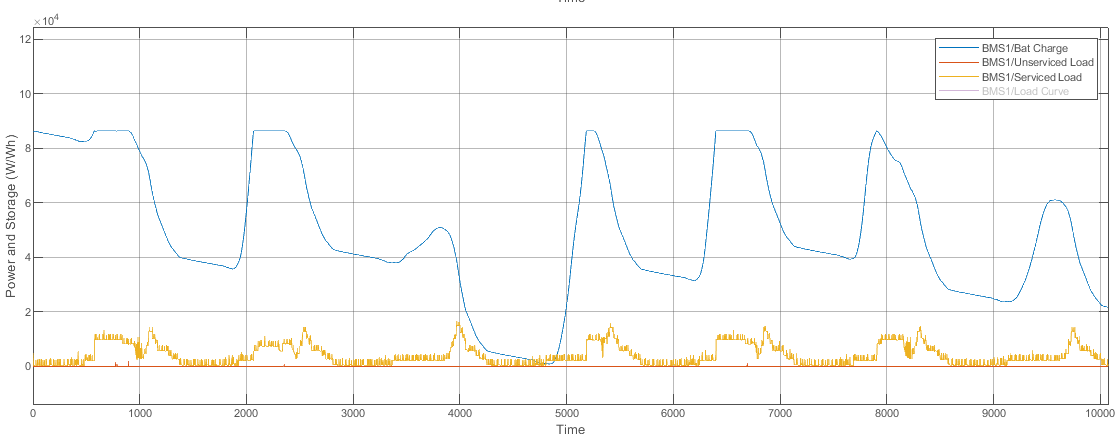
\includegraphics[width=\textwidth]{inc/controlled_charge.png}
    \caption{}
    \label{fig:}
\end{figure}

\newpage
\section{Appendix A: MATLAB Function Controller}
\label{ap:matlab}
\lstinputlisting{inc/controller.m}

\section{Appendix B: Full and Internal Model}
\label{ap:model}
    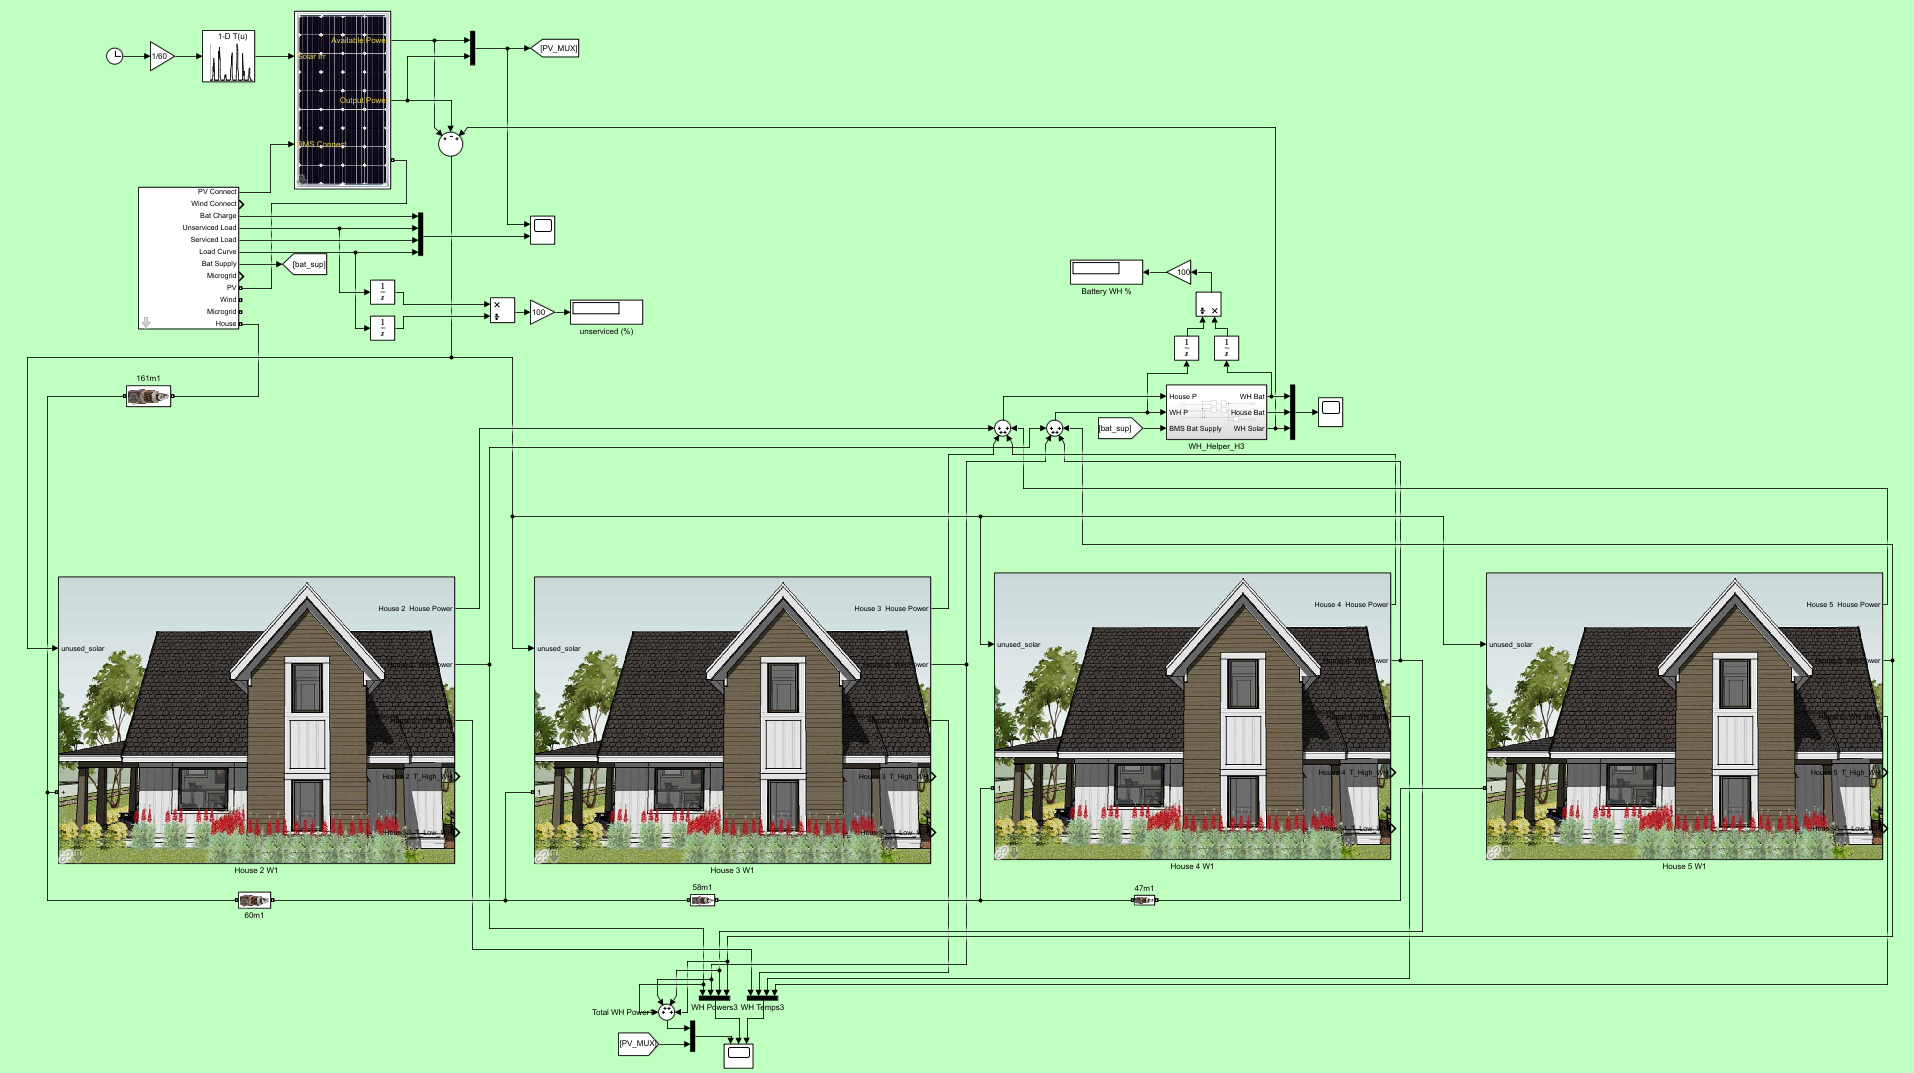
\includegraphics[width=\textwidth]{inc/uGrid_model.png}
    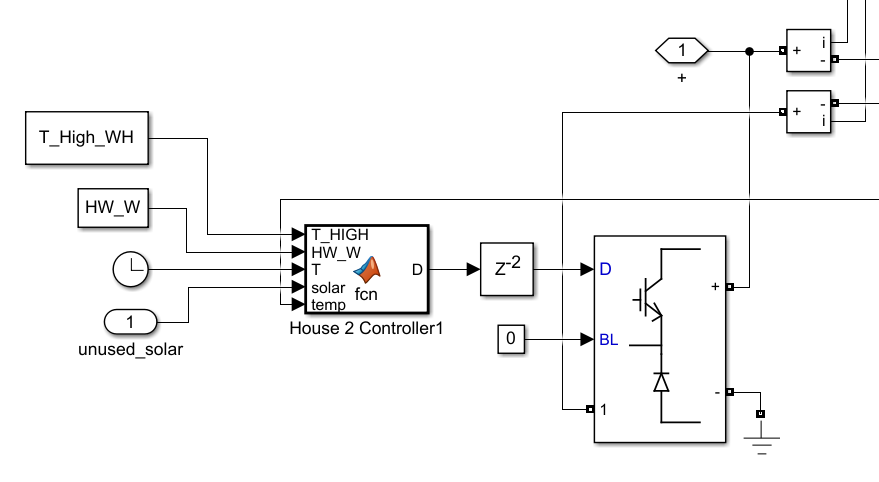
\includegraphics[width=\textwidth]{inc/controller_model.png}

\newpage
\nocite{*}
\bibliography{ref}
\bibliographystyle{IEEEtran}
\end{document}
